% 2002 年全国新课程理科第 18 题甲：正三棱柱
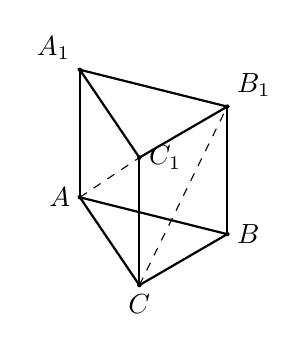
\begin{tikzpicture}[>=stealth,scale=0.72]
  \coordinate (A) at (0,0);
  \coordinate (B) at (2.6,-0.65);
  \coordinate (C) at (1.05,-1.55);
  \coordinate (Aone) at (0,2.25);
  \coordinate (Bone) at (2.6,1.60);
  \coordinate (Cone) at (1.05,0.70);
  \draw[thick] (A)--(B)--(C)--cycle;
  \draw[thick] (Aone)--(Bone)--(Cone)--cycle;
  \draw[thick] (A)--(Aone) (B)--(Bone) (C)--(Cone);
  \draw[dashed] (A)--(Cone) (C)--(Bone);
  \fill (A) circle (1.1pt) node[left] {$A$};
  \fill (B) circle (1.1pt) node[right] {$B$};
  \fill (C) circle (1.1pt) node[below] {$C$};
  \fill (Aone) circle (1.1pt) node[above left] {$A_1$};
  \fill (Bone) circle (1.1pt) node[above right] {$B_1$};
  \fill (Cone) circle (1.1pt) node[right] {$C_1$};
\end{tikzpicture}
